%File: supp.tex (AAAI-2026 supplementary material, anonymous)
\def\aaaianonymous{true}

\documentclass[letterpaper]{article} % DO NOT CHANGE THIS
\usepackage[submission]{aaai2026}  % DO NOT CHANGE THIS
\usepackage{times}  % DO NOT CHANGE THIS
\usepackage{helvet}  % DO NOT CHANGE THIS
\usepackage{courier}  % DO NOT CHANGE THIS
\usepackage[hyphens]{url}  % DO NOT CHANGE THIS
\usepackage{graphicx} % DO NOT CHANGE THIS
\urlstyle{rm} % DO NOT CHANGE THIS
\def\UrlFont{\rm}  % DO NOT CHANGE THIS
\usepackage{natbib}  % DO NOT CHANGE THIS
\usepackage{caption} % DO NOT CHANGE THIS
\frenchspacing  % DO NOT CHANGE THIS
\setlength{\pdfpagewidth}{8.5in} % DO NOT CHANGE THIS
\setlength{\pdfpageheight}{11in} % DO NOT CHANGE THIS

\usepackage{amsmath}
\usepackage{amssymb}
\usepackage{amsthm}
\usepackage{booktabs}
\usepackage{makecell}
\usepackage{pifont}

\pdfinfo{
/TemplateVersion (2026.1)
}

\setcounter{secnumdepth}{0}

\newcommand{\silr}{\textsc{SiLR}}
\newcommand{\psione}{\psi_1}
\newcommand{\psitwo}{\psi_2}
\newcommand{\psithree}{\psi_3}

\title{\silr{}: Structure-Preserving Admission and Process Reward for LLM Tool Agents\\Supplementary Material}
\author{Anonymous Submission}
\affiliations{}

\begin{document}
\maketitle

\noindent This supplement collects material referenced from the main paper: the full attack-family constructions (\S A), full proofs of all propositions (\S B), the $\alpha$-window sweep and cross-domain generalization (\S C), and the extended process-reward study (\S D). Section, equation, proposition, and table numbers prefixed ``main'' refer to the main paper.

\section{A. Attack-Family Constructions}
\label{supp:attacks}

We implement four attack families under the compromised-prompt/compromised-observation capability class of the main paper. \emph{Prompt injection} (C1): a high-priority operator-impersonating override that pushes an aggressive fixed setpoint. \emph{Observation poisoning} (C2): a fabricated ``all readings nominal'' stanza spliced into every observation, contradicting the violation list the verifier re-derives from the live simulator. \emph{Stall} (C1): near-no-op setpoints that stay admissible while never recovering; a ``stall-RAG'' variant instructs the same behavior through a poisoned retrieval context. \emph{Magnitude redistribution} (C1/C2): driving a single retained branch toward failure while holding the overloaded-branch set and aggregate penalty within nominal bounds, masking per-branch overload behind nominal aggregate- and support-level readings.

The mini-suite (main RQ4) runs the three attack families in four configurations---prompt injection, observation poisoning, and stall in plain and RAG forms---across the three mined multi-action scenarios at $N{=}5$ per configuration, plus a matched benign control ($60$ attack $+\,15$ benign $=75$ episodes). Across the $60$ attack episodes the verifier produces $0/60$ attack success, false recovery, and material worsening (Wilson 95\% CI $[0.00,0.06]$), with $0/15$ on the benign control; under prompt injection the rejection rate climbs sharply. The fourth family, magnitude redistribution, is evaluated against competing gates in the $120$-case redistribution suite of main Fig.~4: by concentrating severity on a single retained branch while preserving the overloaded-branch set and holding the aggregate penalty within nominal bounds, its cases slip past aggregate- and support-level gates ($43/120$ and $11/120$) while the per-branch test $\psithree$ rejects every one.

\paragraph{Strong-scalar baselines on the full witness pool.}
Beyond the balanced $120$-case suite, we enumerate \emph{every} physically-unsafe one-step action in each domain---$558$ in ANM, $11{,}311$ in CityLearn (the latter under an independent state-of-charge/feeder-overload oracle, verifier-level, no LLM in the loop)---and evaluate all five gates (Table~\ref{tab:fullpool}). The denominator is a constructed witness pool, not a natural-attack frequency, and absolute breach counts reflect each pool's category composition; they are \emph{not} comparable across gates or domains. The one domain-invariant statement is that the full product order admits zero in both. The strongest scalar projections fail on the Prop.~1 antichain in both domains: in ANM all $46$ sup-norm breaches are support expansions with $\max_i\sigma_i$ non-increasing; in CityLearn $6670$ of the $6761$ sup-norm breaches are the same support-expansion class (the new branch a battery or feeder), confirming the mechanism in a second physical system.

\begin{table}[h]
\centering
\caption{Unsafe admissions on the full physically-unsafe witness pool (verifier-level enumeration; counts only---rates reflect per-pool category mix and are not compared across gates or domains). Only the full product order is clean in both domains.}
\label{tab:fullpool}
\footnotesize
\begin{tabular*}{\columnwidth}{@{\extracolsep{\fill}}lcc@{}}
\toprule
Gate & ANM ($N{=}558$) & CityLearn ($N{=}11{,}311$) \\
\midrule
Scalar---aggregate $\sum_i\sigma_i$ & $108$ & $7204$ \\
Scalar---sup-norm $\|\sigma\|_\infty$ & $46$ & $6761$ \\
Scalar---lexicographic $(|S|,\sum_i\sigma_i)$ & $88$ & $7650$ \\
Support-only (Grid-Agent $\psione\wedge\psitwo$) & $258$ & $432$ \\
\textbf{Full SiLR} ($\psione\wedge\psitwo\wedge\psithree$) & $\mathbf{0}$ & $\mathbf{0}$ \\
\bottomrule
\end{tabular*}
\end{table}

\section{B. Proofs}
\label{supp:proofs}

\paragraph{Proposition~1 (Scalarization gap).}
Any scalar surrogate $f:(S,\sigma)\to\mathbb{R}_{\ge0}$ composes the vector-valued violation state with a total order. The pair $\Phi(s)=(\{A\},2\delta e_A)$, $\Phi(s')=(\{A,B\},0.9\delta(e_A{+}e_B))$ forms a $\preceq$-antichain: $S(s')\not\subseteq S(s)$ blocks $s'\preceq s$, while $\sigma_A(s)=2\delta>0.9\delta=\sigma_A(s')$ blocks $s\preceq s'$. Because $f$ maps both into the totally ordered $\mathbb{R}_{\ge0}$, exactly one of $f(s)\le f(s')$ or $f(s')\le f(s)$ holds (or both, if equal), so for any slack $\eta\ge0$ the gate admits at least one of the two transitions, each non-improving under $\preceq$ (one introduces branch $B$; the other inflates $\sigma_A$). For the canonical aggregate $P=\sum_i\sigma_i$, $P(s')=1.8\delta<2\delta=P(s)$, so $P(s')\le(1{+}\eta)P(s)$ for all $\eta\ge0$ and no slack removes the acceptance of $s\to s'$. The argument depends only on $\preceq$ admitting an antichain, hence applies to every scalar surrogate. $\square$

\paragraph{Proposition~2 (Admission invariant).}
By induction on $t$. Base: trivially $S(s_0)\subseteq S(s_0)$ and $\sigma_i(s_0)\le\alpha^0\sigma_i(s_0)$. Step: an admitted action passes $\psitwo\wedge\psithree$ on the shadow, and shadow fidelity makes the live post-state equal the shadow, so $S(s_{t+1})\subseteq S(s_t)$ (giving $S(s_{t+1})\subseteq S(s_0)$ by the inductive hypothesis) and $\sigma_i(s_{t+1})\le\max(\alpha\sigma_i(s_t),\sigma_i(s_t)+\varepsilon)\le\alpha\sigma_i(s_t)+\varepsilon$ for all $i\in S(s_t)$ (and $\sigma_i\equiv0$ off $S(s_t)$). Unrolling $\sigma_i(s_{t+1})\le\alpha\sigma_i(s_t)+\varepsilon$ gives $\sigma_i(s_t)\le\alpha^{t}\sigma_i(s_0)+\varepsilon\sum_{j=0}^{t-1}\alpha^{j}=\alpha^{t}\sigma_i(s_0)+\varepsilon\tfrac{\alpha^{t}-1}{\alpha-1}$; at $\alpha{=}1$ the bound reads $\sigma_i(s_0)+t\varepsilon$. Neither step uses any property of the action source, so the support invariant ($\alpha$-free) holds for any gated policy, including a compromised LLM. The severity term is a worst-case per-step drift envelope, not a descent guarantee: convergence to $S=\emptyset$ depends on proposal quality. $\square$

\paragraph{Proposition~3 (Advantage collapse under scalarization).}
Immediate from the definitions. With $B$ concurrent violation branches, the count delta of cleared violations ranges over $\{0,\dots,B\}$, taking at most $B{+}1$ distinct values; hence every action pair within a count-equivalence class receives identical immediate reward and there is no step-level advantage separation between them. Along a continuous partial reduction of any single branch's severity that does not eliminate it, $|S|$ is unchanged, so the count reward is piecewise constant---zero gradient except at the discrete elimination points. The graded geometric reward's severity term is strictly monotone in that same reduction, so it retains a nonzero advantage signal everywhere on the continuum. Empirically the flat fraction is $98\%$ of the continuous action range. $\square$

\section{C. Robustness and Cross-Domain Generalization}
\label{supp:gen}

\paragraph{$\alpha$-window sweep.}
Recovery holds across an $\alpha$-window: $15/15$ for $\alpha\in[1.05,1.20]$ and $14/15$ at $\alpha{=}1.02$ ($N{=}5$), consistent with the $\alpha$-free support invariant (Prop.~2); the magnitude guard $\psithree$ tightens as $\alpha\to1$ without disturbing support-driven recovery. The full $24$-scenario band (main Table~2) and the cross-family replication (main Table~3) are reported in the main paper.

\paragraph{Cross-domain (CityLearn).}
The full cross-domain replication is reported in the main paper (Table~3, RQ5): the gate semantics recur in CityLearn building-energy dispatch~\citep{citylearn} over three district battery-storage scenarios (CL-1--CL-3; state-of-charge floor/ceiling and feeder-export limits, $\Phi$ indexed by the violating building or feeder). The one model-dependent completion gap is Gemma-3-12B on CL-2: the gate admits every Gemma proposal there (all \texttt{SAFE\_PROGRESS}, zero rejections), so admission ports intact, but its monotone steps stall short of the terminal action other models reach---completion tracks proposal strength, not gate semantics.

\section{D. The Verifier as a Process Reward: Extended Analysis}
\label{supp:reward}

\paragraph{Setup.}
We fine-tune Qwen3-8B with LoRA on the $9$ hardest multi-action ANM scenarios (greedy decoding, without chain-of-thought). Three reward arms share the same structured rollout gate and differ only in the reward signal: \textbf{Geometric} rewards descent in the product order over $\Phi=(S,\sigma)$; \textbf{Count} rewards the count-delta of cleared violations; and a \textbf{Verdict-only} ablation strips the geometric component, leaving only the verdict ladder. We evaluate the checkpoint after the second GRPO~\citep{deepseekmath2024grpo,lightman2024prm} iteration, pooled over $5$ training seeds (Table~\ref{tab:reward}). On a separate $15$-scenario held-out set, the count reward does not transfer---its gated recovery ($0.80$) falls below even the untrained base's ($0.87$)---whereas only the geometric reward retains recovery once the gate is removed.

\begin{table}[t]
\centering
\caption{Verifier-as-reward on the $9$ hardest ANM scenarios ($5$ seeds pooled; recovery [Wilson 95\% CI]). \emph{Ungated} recovery (gate removed at eval) measures internalization: only the full geometric reward stays above the untrained base.}
\label{tab:reward}
\footnotesize
\setlength{\tabcolsep}{5pt}
\begin{tabular*}{\columnwidth}{@{\extracolsep{\fill}}lccc@{}}
\toprule
Reward (signal) & gated & \textbf{ungated} & steps$\downarrow$ \\
\midrule
base (no LoRA) & $0.778$ & $0.778$ & $4.71$ \\
\textbf{Geometric} ($\Phi$ descent) & $\mathbf{0.956}$ & $\mathbf{0.844}$ {\scriptsize[0.71,0.92]} & $\mathbf{3.64}$ \\
Verdict-only (ladder) & $0.889$ & $0.733$ {\scriptsize[0.59,0.84]} & $4.08$ \\
Count (count-delta) & $0.889$ & $0.667$ {\scriptsize[0.52,0.79]} & $3.84$ \\
\bottomrule
\end{tabular*}
\end{table}

\paragraph{Reward formulas.}
All arms share one verdict scaffold and differ only in how an admitted \texttt{SAFE\_PROGRESS} step is scored. For a step from pre-state $s$ to shadow post-state $\hat s$ with verdict $v$,
\begin{equation}
r(s,\hat s)=
\begin{cases}
1+\tfrac12\,\bar m(\hat s) & v=\texttt{PASS}\\[1pt]
\rho_{\bullet}(s,\hat s) & v=\texttt{SAFE\_PROGRESS}\\[1pt]
-\max\!\big(0.3,\,c_{\mathrm{sev}}(\hat s)\big) & v=\texttt{FAIL}\\[1pt]
-1 & v=\texttt{ERROR,}
\end{cases}
\label{eq:reward-scaffold}
\end{equation}
where $\bar m\in[0,1]$ is the mean normalized constraint margin and $c_{\mathrm{sev}}\in\{0.3,0.6,1.0\}$ grades the worst residual violation (warning/violation/critical); a fixed step cost $0.05$ is subtracted from every step and a terminal recovery bonus $+1$ is added at the trajectory level, both shared across arms. Writing $S,\hat S$ for the pre/post overloaded-branch supports with per-branch severities $\sigma_k,\hat\sigma_k$, $E=S\setminus\hat S$ for the eliminated branches, $U=S\cap\hat S$ for the surviving ones, and $f\in F$ for the constraint families partitioning $S$, the three \texttt{SAFE\_PROGRESS} scorings are
\begin{align}
\rho_{\mathrm{geom}} &= \tfrac{W_2}{|F|}\!\sum_{f\in F}\!\frac{\sum_{k\in E\cap f}\sigma_k}{\sum_{k\in f}\sigma_k}
+\tfrac{W_3}{|F|}\!\sum_{f\in F}\!\frac{\sum_{k\in U\cap f}\max(0,\sigma_k-\hat\sigma_k)}{\sum_{k\in f}\sigma_k}
\nonumber\\[-1pt]
&\quad-\,W_d\,\min\!\Big(1,\,\max_{k\in U}\tfrac{\max(0,\,\hat\sigma_k-\sigma_k)}{\sigma_k}\Big),
\label{eq:rho-geom}\\[2pt]
\rho_{\mathrm{count}} &= \frac{|S|-|\hat S|}{|S|},
\qquad
\rho_{\mathrm{verdict}} \equiv 0.5,
\label{eq:rho-count}
\end{align}
with weights $(W_2,W_3,W_d)=(0.6,0.3,0.3)$, so severity-weighted support elimination ($\psi_2$) outranks per-branch severity polishing ($\psi_3$), echoing the admission product order; the third term penalizes any surviving branch driven worse. The geometric arm normalizes \emph{within} each family and averages families with equal weight, so no high-$\sigma$ family hijacks the signal; for a single family it reduces exactly to $\Sigma\sigma$-normalization, leaving the single-type ANM result unchanged. A count-preserving magnitude reallocation ($S{=}\hat S$) earns $\rho_{\mathrm{geom}}\!\approx\!0$ and is debited by the drift term, yet is invisible to $\rho_{\mathrm{count}}$; the \textbf{Verdict-only} arm flattens $\rho$ to a constant, keeping the \texttt{PASS}${>}$\texttt{SAFE\_PROGRESS}${>}$\texttt{FAIL} ladder while discarding within-step geometry. The failure-class study's severity scalar instead uses the total-severity fraction $\rho_{\mathrm{sev}}=\big(\sum_{k\in S}\sigma_k-\sum_{k\in\hat S}\hat\sigma_k\big)/\sum_{k\in S}\sigma_k$, which retains magnitude but collapses the physically incomparable families into one dimension.

\paragraph{Reward-layer fidelity controls.}
The reward-layer comparison of the main paper (geometric confusion $0.000$ vs.\ $0.25$ for count over $24/24$ scenarios) is stable under four controls (Fig.~\ref{fig:reward-controls}). \emph{(i) On-policy distribution.} Scoring confusion on the states visited under three rollout policies---greedy on the geometric reward, greedy on the count reward, and uniform random---keeps the geometric reward at $0.000$ while count ranges $0.21$--$0.22$, so the separation is a property of the reward rather than of a chosen visitation. \emph{(ii) Complexity scaling.} On controlled trap states with $B$ simultaneous violation branches, count confusion grows from $0.347$ at $B{=}2$ to $0.465$ at $B{=}10$ (Pearson $r{=}0.889$) as more distinct actions collapse onto the same count-delta level, while the geometric reward stays at $0.000$: the representational gap widens with problem complexity. \emph{(iii) Exactness.} A learned model approximating the geometric reward inherits approximation noise; perturbing it by Gaussian noise of standard deviation $s\sigma$ raises its mis-ordering rate from $0.011$ ($s{=}0$, the deterministic simulator) past the count projection's $0.157$ only once $s$ exceeds ${\approx}0.8$---the margin the simulator's exactness affords over an approximate process reward. \emph{(iv) Exploit resistance.} Fidelity also bounds how easily the reward is gamed: a binary admit/reject reward pays $+0.5$ for both a \emph{stall} (an admitted no-op, $\hat s{=}s$) and a \emph{drift} (a count-preserving reallocation that worsens a branch), so an $8$-step stall accrues $4.0$ against $1.5$ for recovering in three steps, while the count reward is indifferent to drift; the severity-scalar and geometric rewards both score ${\approx}0$ on a stall and penalize drift. Resistance to both hacks rises with the constraint geometry the reward preserves.

\begin{figure*}[t]
\centering
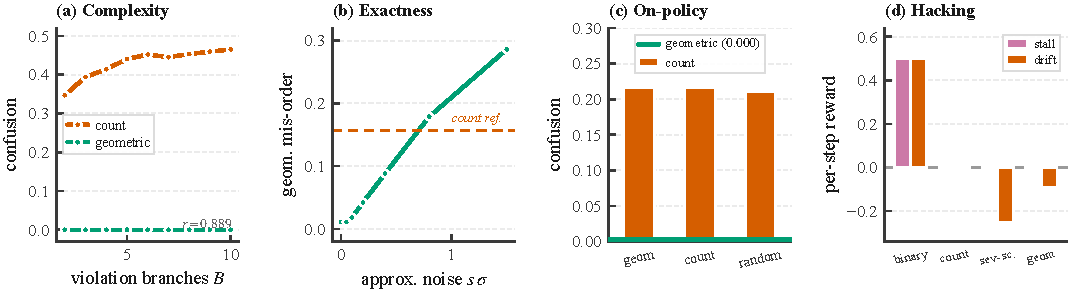
\includegraphics[width=0.97\textwidth]{figures/cand_reward_controls.pdf}
\caption{Reward-layer fidelity controls. (a)~Reward-level confusion grows with the number of simultaneous violation branches $B$ for the count reward (Pearson $r{=}0.889$) while the geometric reward stays at $0.000$. (b)~A learned model approximating the geometric reward must keep its approximation noise below $s{\approx}0.8\,\sigma$ to retain its advantage over the count projection. (c)~The fidelity gap holds on states visited under three rollout policies (geometric confusion $0.000$ throughout; count $0.21$--$0.22$). (d)~A binary admit/reject reward pays $+0.5$ for both stall and drift; the count reward is blind to drift, which the severity-scalar and geometric rewards penalize.}
\label{fig:reward-controls}
\end{figure*}

\paragraph{The multi-family failure class.}
When several physically incomparable violation families are active at once, any scalar reward must collapse the product order into one dimension, and the representational gap of Prop.~1 reappears in training dynamics as advantage collapse (Prop.~3). We run two controlled mechanism-isolation training-dynamics analyses~\citep{krakovna2020specification}, each a minimal multi-family recovery regime isolating one component of the geometry, with GRPO on the unmodified reward functions ($16$ training seeds each; trained recovery in main Table~4). In the \emph{$\sigma$-heterogeneity regime} (one large-$\sigma$ family, one small-$\sigma$ family whose violation is urgent), the severity scalar is hijacked by raw magnitude---it chases the large family and recovers $0\%$---while per-family normalization makes the urgent family's elimination worth a full family and recovers $100\%$. In the \emph{coupling regime} (clearing the large family drifts the small family toward an irreversible limit), the count reward is blind to the drift its own actions cause and trains to $12\%$; the drift-aware geometric reward trains to $100\%$. Restoring the drift term rescues count in the coupling regime ($1.00$) but cannot restore cross-family priority ($0.80$ under $\sigma$-heterogeneity), and the severity scalar fails in both.

The $\sigma$-heterogeneity sweep (main Fig.~5(b)) shows the failure is not an artifact of a chosen operating point: it emerges at $\sigma_L/\sigma_S\!\approx\!4$, saturates from $8$ onward (CityLearn's measured heterogeneity is $286$), and vanishes in the homogeneous limit. The separation holds across the full $4{\times}4$ coupling--floor grid (Fig.~\ref{fig:failgrid}): geometric $\ge0.97$ in all $16$ cells, count $\le0.42$ in $15$; the single benign cell is the setting where coupling is too weak to threaten the fragile family. An MLP policy reproduces the same ordering ($1.00/0.13/0.05$ for geometric/count/severity-scalar), so the pattern is not specific to the policy class.

\begin{figure*}[t]
\centering
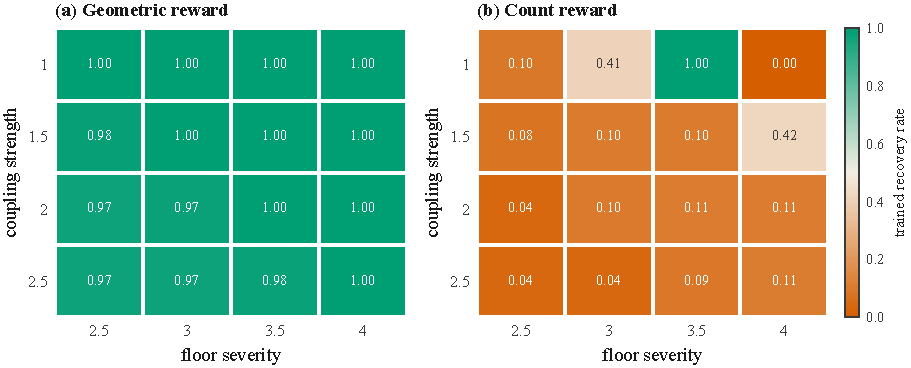
\includegraphics[width=0.84\textwidth]{figures/cand_failclass_heatmap.pdf}
\caption{Trained recovery across the $4{\times}4$ coupling--floor grid. The geometric reward recovers $\ge0.97$ in all $16$ cells; the count reward collapses ($\le0.42$) in $15$ of $16$, recovering only the single benign cell $(\sigma_L/\sigma_S, c_{\text{floor}}){=}(1.0,3.5)$ where coupling is too weak to threaten the fragile family.}
\label{fig:failgrid}
\end{figure*}

\paragraph{The mechanism at full scale.}
Training Qwen3-8B with GRPO on the multi-family CityLearn suite (four buildings, $\sigma$-het $286$) reproduces the mechanism in a second, larger system and exposes a credit-assignment requirement: trajectory-return credit is required to propagate delayed cross-family consequences, since a per-step z-score cannot assign the cost of flooring the battery family back to the early step that caused it. With trajectory-return credit the trained policies separate along the axis Prop.~3 predicts. Across seeds the geometric reward's advantage signal tracks the true one-step action value at Spearman $\rho{=}0.96$ versus $0.79$ for count, and after training the count arm leaves the battery family at $14\%$ higher residual severity than the geometric arm at the same violation count---the signature of a severity-blind signal.

\bibliography{refs}

\end{document}
